\section{Application(s)}

The WellBean was designed to be used in an office space, where every employee has a desk with power plugs, sufficient space for an additional device with the size of an Arduino on the desk, and an internet connection. In a real-world setup, multiple end devices would be connected to a Raspberry Pi serving as the gateway to «the Cloud».

The data collected could be used then by a data science team to gain insight into optimal workplace conditions, both for the team as a whole, as well as for the individual members of the team, which might have different notions of good environmental conditions. Figure \imgref{fig:beansalad} shows such a possible setup.

\begin{figure}
	\centering
	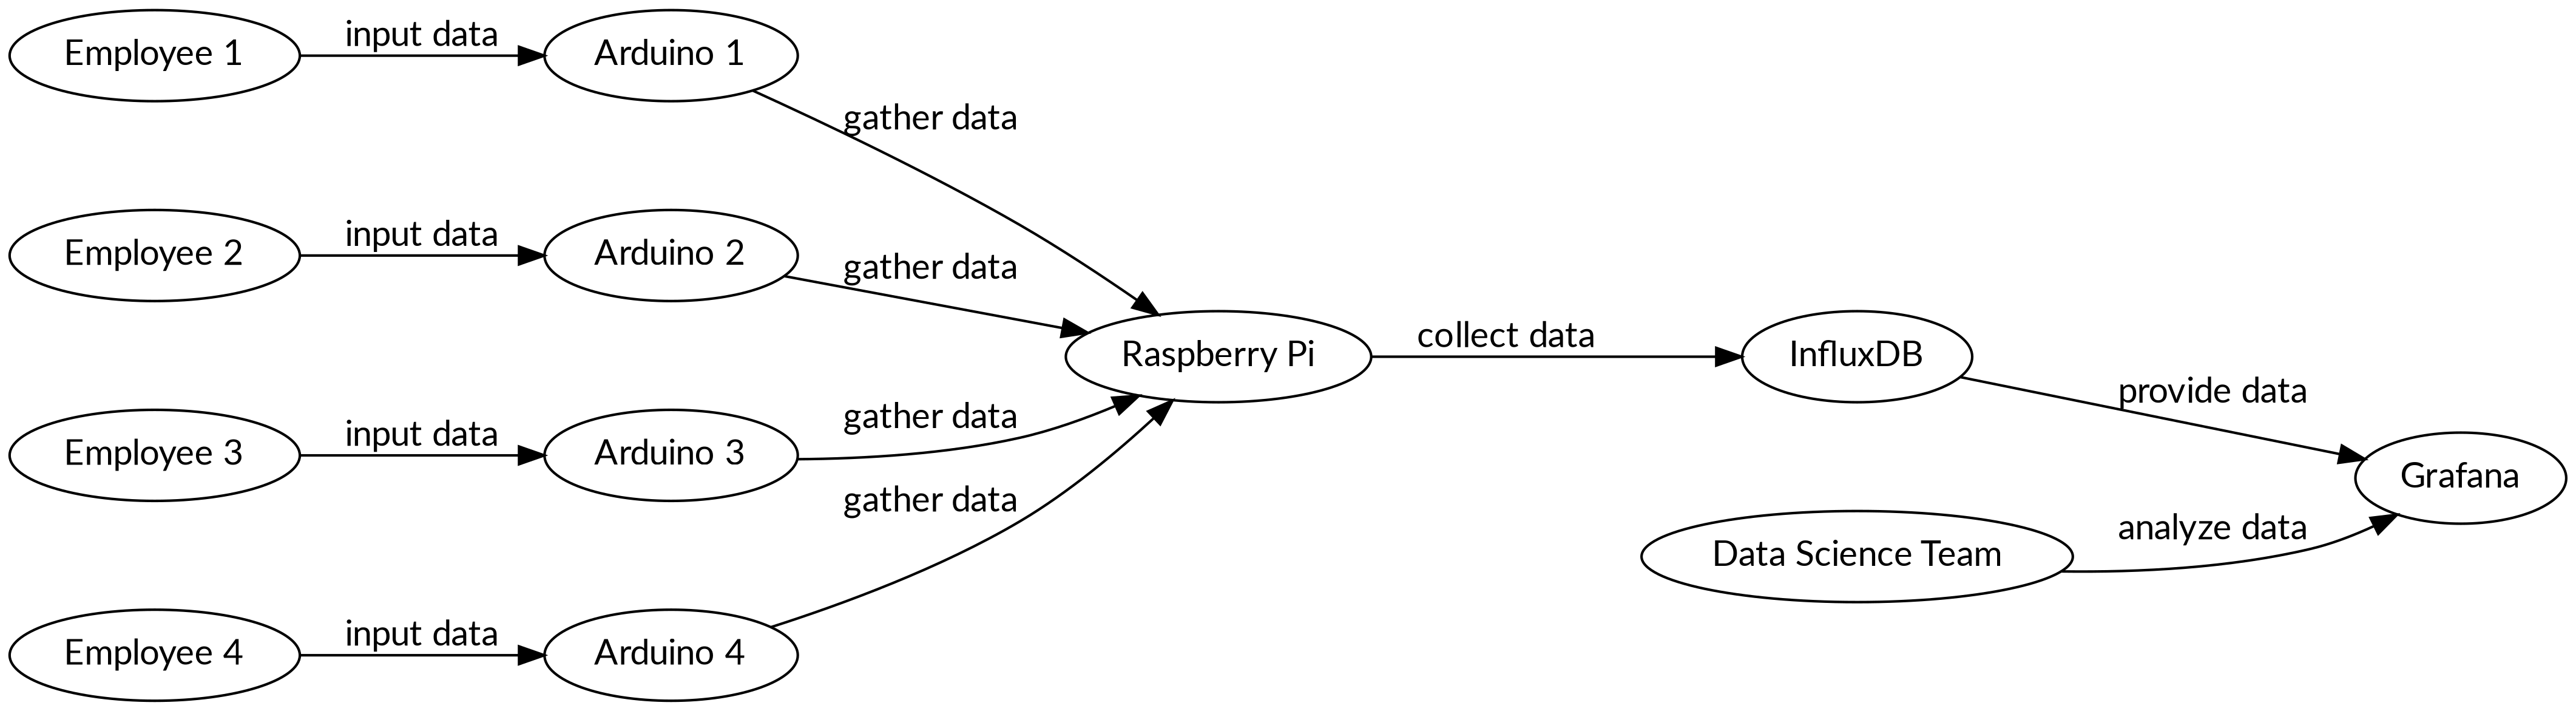
\includegraphics[width=\linewidth]{applications.png}
	\caption{Possible Future Application for the WellBean (Codename: «BeanSalad»)}
	\label{fig:beansalad}
\end{figure}
